
%%%%%%%%%%%%%%%%%%%%%%%%%%%%%%%%%%%%%%%%%%%%%%%%%%%%%%%%%%%%%%%%%%%%%%%%%%%%%%%%
%
% Numerical Methods
%
%%%%%%%%%%%%%%%%%%%%%%%%%%%%%%%%%%%%%%%%%%%%%%%%%%%%%%%%%%%%%%%%%%%%%%%%%%%%%%%%

\section{Numercial Methods}
\label{sec:2lpt--methods}

%%%%%%%%%%%%%%%%%%%%%%%%%%%%%%%%%%%%%%%%%%%%%%%%%%%%%%%%%%%%%%%%%%%%%%%%%%%%%%%%



%~~~~~~~~~~~~~~~~~~~~~~~~~~~~~~~~~~~~~~~~~~~~~~~~~~~~~~~~~~~~~~~~~~~~~~~~~~~~~~~
% Simulations
%~~~~~~~~~~~~~~~~~~~~~~~~~~~~~~~~~~~~~~~~~~~~~~~~~~~~~~~~~~~~~~~~~~~~~~~~~~~~~~~


We use the \nbody\ tree/SPH code \gadgettwo\ \citep{2001NewA....6...79S, 2005MNRAS.364.1105S} to evolve six dark matter--only cosmological volumes from $z_{start} = 300$ to $z = 6$ in a $\rm \Lambda CDM$ universe.  Each simulation is initialized using WMAP-5 \citep{2009ApJS..180..330K} parameters.  For each of the three simulation pairs, we directly compare \lpt\ and \za\ by identically sampling the CMB transfer function and displacing the initial particle positions to the same starting redshift using \lpt\ and \za.  The three sets of simulations differ only by the initial phase sampling random seed.  Each volume contains $512^{3}$ particles in a 10 $h^{-1}$ Mpc box.  Following \citet{2010ApJ...715..104H}, we choose conservative simulation parameters in order to ensure high accuracy in integrating the particle positions and velocities.  We have force accuracy of 0.002, integration accuracy of 0.00125, and softening of $0.5\ h^{-1}\ \mathrm{kpc}$, or $1 / 40$ of the initial mean particle separation.  We use a uniform particle mass of $5.3 \times 10^{5} h^{-1} \Msun$.  Full simulation details are discussed in \citet{2012ApJ...761L...8H}.

One facet often overlooked when setting up an \nbody\ simulation is an appropriate starting redshift, determined by box size and resolution \citep{2007ApJ...671.1160L}.  As \lpt\ more accurately displaces initial particle positions and velocities, initialization with \lpt\ allows for a later starting redshift compared with an equivalent \za-initialized simulation.  However, many \za\ simulations do not take this into account, starting from too late an initial redshift and not allowing enough $e$-foldings to adequately dampen away numerical transients \citep{2006MNRAS.373..369C, 2010MNRAS.403.1859J}.  In order to characterize an appropriate starting redshift, the relation between the initial rms particle displacement and mean particle separation must be considered.  The initial rms displacement $\Delta_{\mathrm{rms}}$ is given by
\begin{equation}
	\Delta_{\mathrm{rms}}^{2} = \frac{4 \pi}{3} \int_{k_{f}}^{k_{\mathrm{Ny}}} P(k, z_{\mathrm{start}}) \dd k,
\end{equation}
where $k_{f} = 2 \pi / L_{\mathrm{box}}$ is the fundamental mode, $L_{\mathrm{box}}$ is the simulation box size, $k_{\mathrm{Ny}} = \frac{1}{2} N k_{f}$ is the Nyquist frequency of an $N^{3}$ simulation, and $P(k, z_{\mathrm{start}})$ is the power spectrum at starting redshift $z_{\mathrm{start}}$.  In order to avoid the ``orbit crossings'' that reduce the accuracy of the initial conditions, $\Delta_{\mathrm{rms}}$ must be some factor smaller than the mean particle separation $\Delta_{p} = L_{\mathrm{box}} / N$ \citep{2012ApJ...761L...8H}.  For example, making orbit crossing a $\sim 10 \sigma$ event imposes $\Delta_{\mathrm{rms}} / \Delta_{p} = 0.1$.  However, for small-volume, high-resolution simulations, this quickly leads to impractical starting redshifts.  Continuing our example, satisfying $\Delta_{\mathrm{rms}} / \Delta_{p} \sim 0.1$ for a $10 h^{-1}$ Mpc, $512^{3}$ simulation suggests $z_{\mathrm{start}} \approx 799$.  Unfortunately, starting at such a high redshift places such a simulation well into the regime of introducing errors from numerical noise caused by roundoff errors dominating the smooth potential.  A more relaxed requirement of $\Delta_{\mathrm{rms}} / \Delta_{p} = 0.25$, which makes orbit crossing a $\sim 4\sigma$ event, yields $z_{\mathrm{start}} = 300$, which we adopt for this work.  For our small volume, the fundamental mode becomes non-linear at $z \sim 5$, after which, simulation results would become unreliable.  We therefore end our simulations at $z = 6$.




%~~~~~~~~~~~~~~~~~~~~~~~~~~~~~~~~~~~~~~~~~~~~~~~~~~~~~~~~~~~~~~~~~~~~~~~~~~~~~~~
% Rockstar
%~~~~~~~~~~~~~~~~~~~~~~~~~~~~~~~~~~~~~~~~~~~~~~~~~~~~~~~~~~~~~~~~~~~~~~~~~~~~~~~


For each of our six simulations, we use the 6-D phase space halo finder code \rockstar\ \citep{2013ApJ...762..109B} to identify spherical overdensity halos at each timestep.  \rockstar\ follows an adaptive hierarchical refinement of friends-of-friends halos in 6-D phase space, allowing determination of halo properties such as halo mass, position, virial radius, internal energy, and number of subhalos.  \rockstar\ tracks halos down to a threshold of around 20 particles, but we use a more conservative 100 particle threshold for our analysis.  We use all particles found within the virial radius to define our halos and their properties.




%~~~~~~~~~~~~~~~~~~~~~~~~~~~~~~~~~~~~~~~~~~~~~~~~~~~~~~~~~~~~~~~~~~~~~~~~~~~~~~~
% CrossMatch
%~~~~~~~~~~~~~~~~~~~~~~~~~~~~~~~~~~~~~~~~~~~~~~~~~~~~~~~~~~~~~~~~~~~~~~~~~~~~~~~


We identify companion halos between \lpt\ and \za\ simulations based on the highest fraction of matching particles contained in each at any given timestep.  We remove halo pairs where either one or both halos are considered subhalos (i.e. a halo must not be contained within another halo) and pairs with fewer than 100 particles in either \lpt\ or \za.  We are left with approximately 60,000 total halo pairs for our three boxes at $z = 6$.  With halo catalogs matched between simulations, we can compare properties of individual corresponding halos.  To mitigate the effects of cosmic variance on our small volumes, we ``stack'' the three simulation boxes for each initialization method, and combine the halos from each into one larger sample for our analysis.




%~~~~~~~~~~~~~~~~~~~~~~~~~~~~~~~~~~~~~~~~~~~~~~~~~~~~~~~~~~~~~~~~~~~~~~~~~~~~~~~
% Density Profiles
%~~~~~~~~~~~~~~~~~~~~~~~~~~~~~~~~~~~~~~~~~~~~~~~~~~~~~~~~~~~~~~~~~~~~~~~~~~~~~~~


\begin{figure}[tp]
    \centering
    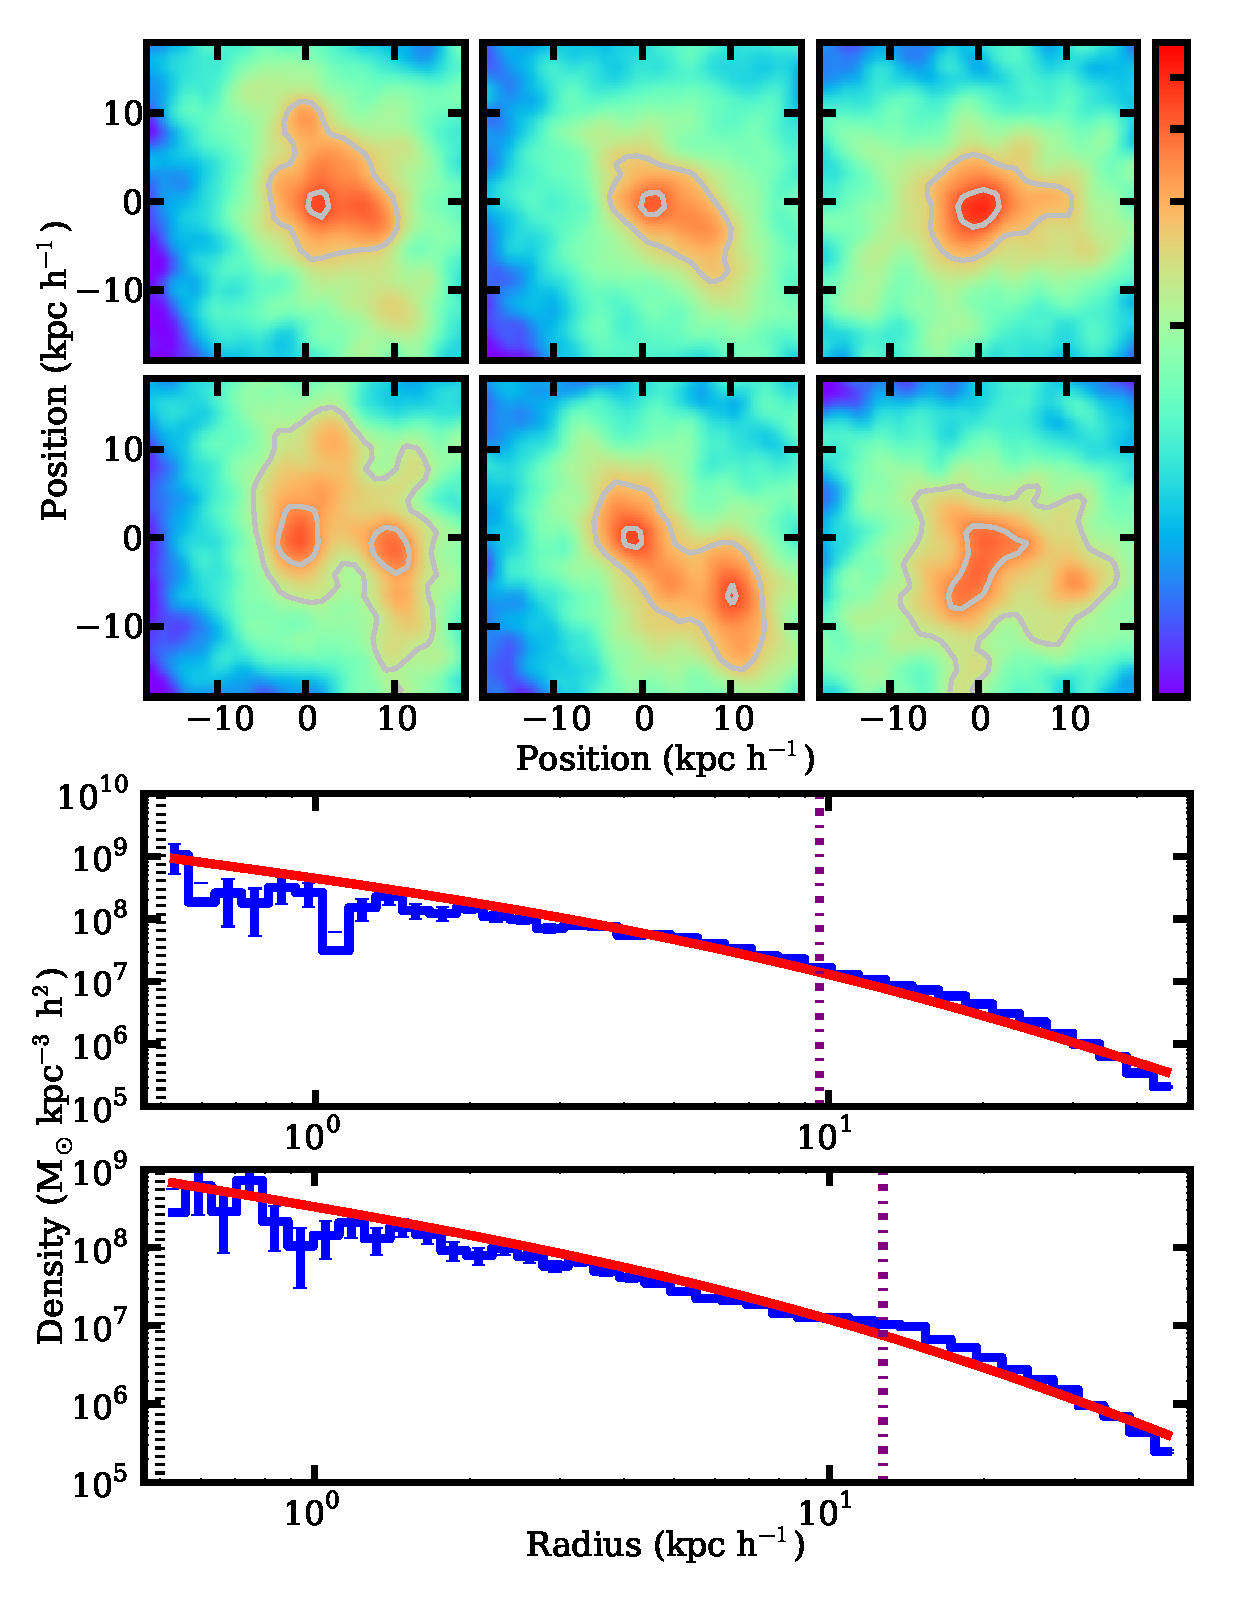
\includegraphics[width=0.9\linewidth]{halo-pair_070_snap061.eps}
	\caption[Comparison of matched \lpt\ and \za\ halos]{\footnotesize \textit{Top two rows:}  Density projections for two matching halos at $z = 6$.  The first and second row are \lpt\ and \za, respectively.  The halos appear to be either undergoing or have recently undergone a major merger.  The \lpt\ halo appears to be more relaxed and further along in the merger process, while the \za\ halo lags behind, still displaying two distinct cores.  The halos have masses of $5.95 \times 10^{9} \textrm{M}_{\odot}$ for \lpt\ and $5.85 \times 10^{9} \textrm{M}_{\odot}$ for \za.  \textit{Bottom two rows:}  Density profiles for the same two halos as above.  NFW profiles are fit to logarithmic radial bins of particle position and are overplotted as red curves.  The purple dot--dash lines mark the scale radii.  The black dotted lines mark the resolution limit of the simulations.}
    \label{fig:halo-pair}
\end{figure}

Halo concentration is derived from \rockstar's output for $R_{s}$ and $R_{\mathrm{vir}}$.  Here, $R_{\mathrm{vir}}$ is the virial radius as defined by \citet{1998ApJ...495...80B}.  Figure~\ref{fig:halo-pair} makes evident the difficulty in fitting density profiles and obtaining concentration measurements for typical realistic halos.  Large substructure, as displayed by the \za\ halo, can disrupt the radial symmetry of the halo and cause significant deviations in the density profile.  Centering can also be an issue in these cases.  Due to these complications, there are a number of approaches for finding halo concentrations \citep{2012MNRAS.423.3018P}, but for consistency, we use the values derived from \rockstar's fitting for our concentration measurements.




%~~~~~~~~~~~~~~~~~~~~~~~~~~~~~~~~~~~~~~~~~~~~~~~~~~~~~~~~~~~~~~~~~~~~~~~~~~~~~~~
% Histograms and Curve Fitting
%~~~~~~~~~~~~~~~~~~~~~~~~~~~~~~~~~~~~~~~~~~~~~~~~~~~~~~~~~~~~~~~~~~~~~~~~~~~~~~~


At each simulation snapshot, we measure and compare a number of parameters for halos in both \lpt\ and \za\ simulations.  For each quantity $q$, we create histograms of $\Delta q$, the normalized difference in $q$ between halos in the \lpt\ and \za\ simulations:
\begin{equation} \label{eq:delta_q}
	\Delta q = \frac{q_{\lpt} - q_{\za}}{q_{\mathrm{avg}}},
\end{equation}
where $q_{\mathrm{avg}} = \frac{1}{2} (q_{\lpt} + q_{\za})$.  The choice of $q_{\mathrm{avg}}$ for normalization allows us to be unbiased in our assumption of which halo better represents the truth, but can mask large differences between individual halos.  We fit each of these $\Delta q$ histograms with a generalized normal distribution \citep{doi:10.1080/02664760500079464} with the probability density function
\begin{equation} \label{eq:generalized_normal}
	f(x) = \frac{ \beta }{2 \alpha \Gamma(1 / \beta)} e^{\left( \left| x - \mu \right| / \alpha \right)^{\beta}},
\end{equation}
where $\mu$ is the mean, $\alpha$ is the scale parameter, $\beta$ is the shape parameter, and $\Gamma$ is the gamma function
\begin{equation} \label{eq:gamma_function}
	\Gamma(t) = \int_{0}^{\infty} x^{t-1} e^{-x} \dd x.
\end{equation}
The shape parameter $\beta$ is restricted to $\beta \geq 1$.  This allows the distribution to potentially vary from a Laplace distribution ($\beta = 1$) to a uniform distribution ($\beta = \infty$) and includes the normal distribution ($\beta = 2$).  The distribution has variance
\begin{equation} \label{eq:variance}
	\sigma^{2} = \frac{ \alpha^{2} \Gamma(3/\beta) }{ \Gamma(1/\beta) }
\end{equation}
and excess kurtosis
\begin{equation} \label{eq:kurtosis}
	\gamma_{2} = \frac{ \Gamma(5/\beta) \Gamma(1/\beta) }{ \Gamma(3/\beta)^{2} } - 3.
\end{equation}
The distribution is symmetric, and thus has no skewness by definition.  As such, the values for skew presented below are measured directly from the data.

As our fitting distributions are symmetrical, in order to derive uncertainties for skew, we measure the skew of the distributions for each of our three simulation boxes individually as well as for the single stacked data set.  Uncertainty in skew is then simply the standard deviation of the mean of the skew of the three individual boxes.

Determining the uncertainty in the kurtosis is slightly more involved, as kurtosis is determined by a transformation of the generalized normal distribution's shape parameter $\beta$ according to Equation~\ref{eq:kurtosis}.  Following the standard procedure for propagation of uncertainty, we calculate the standard deviation of the kurtosis:
\begin{align} \label{eq:kurt_err_partial}
    s_{\gamma_{2}} &= \sqrt{ \left( \frac{\diff \gamma_{2}}{\diff \beta} \right)^{2} s_{\beta}^{2} } \\
        &= s_{\beta} \frac{\diff}{\diff \beta} \left[ \frac{\Gamma(5/\beta) \Gamma(1/\beta)}{\Gamma(3/\beta)^{2}} - 3 \right].
\end{align}
The derivative of the gamma function is
\begin{equation} \label{eq:gamma_prime}
    \Gamma'(x) = \Gamma(x) \psi_{0}(x),
\end{equation}
where the digamma function $\digamma$ is the derivative of the logarithm of the gamma function and is given by
\begin{equation} \label{eq:digamma}
    \digamma(x) = \int_{0}^{\infty} \left( \frac{e^{-t}}{t} - \frac{e^{-xt}}{1 - e^{-t}} \right) \dd t
\end{equation}
if the real part of $x$ is positive.  Now, taking the derivative of $\gamma_{2}$ and doing a bit of algebra yields
\begin{equation} \label{eq:kurt_err}
    s_{\gamma_{2}} = s_{\beta} \frac{1}{\beta^{2}} \left( \gamma_{2} + 3 \right) \left[ 6 \digamma(3/\beta) - 5 \digamma(5/\beta) - \digamma(1/\beta) \right],
\end{equation}
with which we can find the uncertainty in the kurtosis given the value and uncertainty of the shape parameter $\beta$ estimated from the least squares fit routine.

In addition to distributions of $\Delta q$, we also consider distributions of
\begin{equation} \label{eq:delta_prime_q}
	\delta q = \frac{q_{\lpt} - q_{\za}}{q_{\za}}
\end{equation}
to better quantify the fraction of halos differing by a given amount between \lpt\ and \za\ simulations.  This is better suited to track the fractional differences between the halo populations and allows us to pose questions like:  how many \lpt\ halos are more massive than their \za\ counterparts by at least a given amount?  However, this function is inherently non-symmetrical, and is only defined for $\delta q \geq -1$ for positive quantities like mass and concentration.  Therefore, in order to count halo pairs that differ by a certain amount, regardless of whether $q$ is larger for the \lpt\ or \za\ halo, we define
\begin{equation} \label{eq:equivalent_q_prime}
	\delta q_{eq} = \frac{1}{\delta q + 1} - 1,
\end{equation}
the value for which a halo pair with a larger $q$ in \za\ would differ by the same factor as a halo pair with a larger $q$ in \lpt.



